\documentclass[tikz,border=2pt]{standalone}
\usepackage{amsmath,amssymb}
\usepackage{tikz}
\usetikzlibrary{arrows.meta}

\begin{document}
% In an eigenbasis (p1, p2) of A = [[2,1],[1,2]] the map is just a stretch along each basis
% direction: coordinates (c1, c2) become (3 c1, 1 c2).
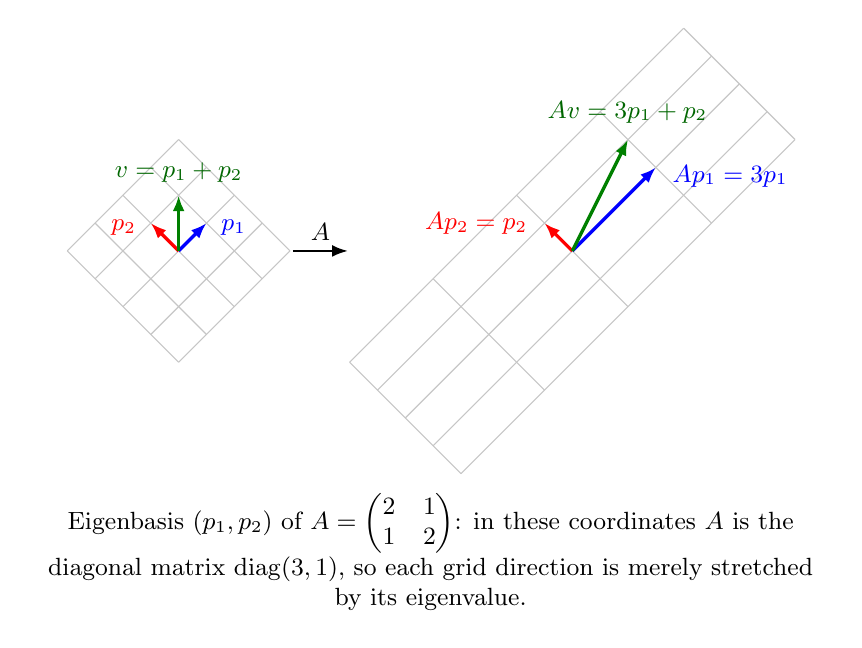
\begin{tikzpicture}[every node/.style={font=\small}, >={Latex[length=2mm]}]
	\begin{scope}[rotate=45]
		\foreach \i in {-2,...,2} {
			\draw[gray!45] (\i*0.5,-1.0) -- (\i*0.5,1.0);
			\draw[gray!45] (-1.0,\i*0.5) -- (1.0,\i*0.5);
		}
		\draw[->, blue, very thick] (0,0) -- (0.5,0);
		\draw[->, red, very thick] (0,0) -- (0,0.5);
		\draw[->, green!50!black, very thick] (0,0) -- (0.5,0.5);
	\end{scope}
	\node[blue, anchor=west] at (0.42,0.3) {$p_1$};
	\node[red, anchor=east] at (-0.42,0.3) {$p_2$};
	\node[green!40!black, anchor=south] at (0,0.75) {$v=p_1+p_2$};
	\draw[->, thick] (1.45,0) -- (2.15,0) node[midway, above] {$A$};
	\begin{scope}[xshift=5.0cm, rotate=45]
		\foreach \i in {-2,...,2} {
			\draw[gray!45] (\i*1.5,-1.0) -- (\i*1.5,1.0);
			\draw[gray!45] (-3.0,\i*0.5) -- (3.0,\i*0.5);
		}
		\draw[->, blue, very thick] (0,0) -- (1.5,0);
		\draw[->, red, very thick] (0,0) -- (0,0.5);
		\draw[->, green!50!black, very thick] (0,0) -- (1.5,0.5);
	\end{scope}
	\node[blue, anchor=west] at (6.15,0.95) {$Ap_1=3p_1$};
	\node[red, anchor=east] at (4.55,0.35) {$Ap_2=p_2$};
	\node[green!40!black, anchor=south] at (5.7,1.5) {$Av=3p_1+p_2$};
	\node[anchor=north, align=flush center, text width=10cm] at (3.2,-2.95) {Eigenbasis $(p_1,p_2)$ of $A=\begin{pmatrix}2&1\\1&2\end{pmatrix}$: in these coordinates $A$ is the diagonal matrix $\operatorname{diag}(3,1)$, so each grid direction is merely stretched by its eigenvalue.};
\end{tikzpicture}
\end{document}
